\documentclass[doc,a4paper,biblatex]{apa7}
\usepackage[utf8]{inputenc}
\usepackage[T1]{fontenc}

\usepackage[american]{babel}
\usepackage{csquotes}

\usepackage[style=apa, backend=biber]{biblatex}
\addbibresource{references.bib}

\usepackage{listings}
\usepackage{xcolor}

\lstdefinestyle{code}{
  basicstyle=\ttfamily\small,
  breaklines=true,
  breakatwhitespace=false,
  frame=single,
  framerule=0.4pt,
  xleftmargin=1em,
  xrightmargin=1em,
  captionpos=b,
  commentstyle=\color{gray},
  keywordstyle=\color{black},
}
\lstset{style=code}

\usepackage{booktabs}

\title{\texttt{shuffle}: A Tool for Generating Quasi-Randomised Stimulus Lists with Sequential Constraints}

\shorttitle{Shuffling List with Sequential Constraints}

\author{Christophe Pallier}
\affiliation{Cognitive Neuroimaging Unit, CNRS INSERM CEA}

\authornote{\addORCIDlink{Christophe Pallier}{0000-0002-3324-666X} Correspondence should be addressed to INSERM, Neurospin, Gif-sur-Yvette, F-91191, France. E-mail: christophe@pallier.org}

\abstract{%
Experimental psychologists routinely need to randomise the order of
trials across participants while avoiding undesirable sequential
patterns---for example, long runs of trials belonging to the same
stimulus category, or target items appearing too close together. We
present \texttt{shuffle-go}, a freely available, cross-platform tool for
generating quasi-randomised sequences that satisfy user-defined
sequential constraints. Input is a plain-text or CSV table whose rows
represent trials and whose columns represent categorical variables
(\textit{e.g.}, stimulus type, response mapping, condition). Two types
of constraint can be imposed on any column: a \textit{maximum-repetition}
constraint limits the number of consecutive rows that may share the same
label, and a \textit{minimum-gap} constraint requires a minimum number of
intervening rows between any two rows sharing the same label. Two
algorithms are provided. The \textit{constructive} algorithm builds a
valid permutation row by row and is fast enough for everyday use. The
\textit{equiprobable} algorithm draws random permutations repeatedly until
one satisfies the constraints, guaranteeing an unbiased sample from the
set of valid permutations; it is slower but preferable when distributional
properties of the randomisation matter. \texttt{shuffle-go} is implemented
in Go and distributed as self-contained binaries for Windows, macOS, and
Linux (both x86-64 and ARM64), requiring no runtime installation. It
offers a command-line interface, two graphical desktop interfaces, an
embeddable Go library, and a Python library. Source code is available at
\url{https://github.com/chrplr/shuffle-go} under the GPLv3 licence.%
}

\keywords{stimulus list randomisation, quasi-randomisation, sequential
  constraints, experiment design, open-source software}


\begin{document}

\maketitle

\newpage


\section{Introduction}
\label{sec:introduction}

A fundamental step in the design of behavioural experiments is
deciding the order in which stimuli are presented to
participants. Fully random ordering, where any of the $n!$
permutations of $n$ trials is equally probable, is simple to implement
but can produce sequences that practically problematic. Long runs of
trials sharing the same category, response key, or difficulty level
are known to affect response times \parencite{luce1986} and can
introduce systematic carry-over effects that confound the variables of
interest. Conversely, in paradigms such as long-term repetition
priming, it is necessary that critical items be separated by a minimum
number of filler trials to prevent short-term repetition effects from
masking the phenomenon under investigation. The practical solution is
\textit{quasi-randomisation}: generating permutations that are random
in a global sense while obeying local sequential constraints. This
requires software that goes beyond a simple shuffle.

We present \texttt{shuffle-go}, the latest in a series of implementations
of this approach (see \textbf{history} below). It is distributed as
self-contained compiled binaries for Windows, macOS, and Linux, requires
no runtime installation, and supports modern platforms including ARM64
(Apple Silicon, Raspberry Pi). It provides both a command-line interface and
graphical desktop applications, an embeddable Go library, and a Python
library.

The closest comparable tool is \texttt{Mix} \parencite{vancasteren2006},
which supports the same two constraint types, that is, maximum consecutive
repetitions and minimum gap between identical labels, across multiple
columns. \texttt{Mix} is widely used and well-validated, but is limited
to Windows, is distributed as a closed-source binary, and provides no
command-line interface or embeddable library. It does not offer an
equiprobable shuffling mode. \texttt{shuffle-go} was designed to address
these limitations while maintaining full compatibility with the same
constraint model.

Other tools take complementary approaches. \textcite{ihrke2011} describe
a genetic-algorithm-based tool for generating trial sequences in priming
paradigms, which handles complex inter-trial dependencies
(\textit{e.g.}, prime--probe relationships across successive trials) that
go beyond simple repetition and gap constraints; this added expressiveness
comes at the cost of greater complexity and longer run times.
\texttt{python-pseudorandom} \parencite{mathot2014}, distributed as part
of the OpenSesame experiment builder ecosystem, provides max-repetition
constraints on single or combined columns in Python, but does not support
min-gap constraints and offers no equiprobable mode. Neither tool provides
a standalone CLI suitable for scripting outside a specific environment.
Table~\ref{tab:comparison} summarises how \texttt{shuffle-go} compares
to these tools.

\begin{table}[ht]
\caption{Feature comparison of quasi-randomisation tools}
\label{tab:comparison}
\small
\begin{tabular}{@{}lccccc@{}}
\toprule
Feature & \texttt{shuffle-go} & Mix & Ihrke \& Behrendt & \texttt{python-pseudorandom} \\
\midrule
Max-repetition constraint   & Yes & Yes & Yes (GA) & Yes \\
Min-gap constraint          & Yes & Yes & Yes (GA) & No  \\
Equiprobable mode           & Yes & No  & No       & No  \\
Command-line interface      & Yes & No  & No       & No  \\
Embeddable library          & Yes & No  & No       & Yes (Python) \\
Cross-platform              & Yes & Windows only & Yes & Yes (Python) \\
Open source                 & Yes & No  & Yes      & Yes \\
No runtime required         & Yes & Yes & No       & No  \\
\bottomrule
\end{tabular}
\end{table}


% -----------------------------------------------------------------------
\section{History}
\label{sec:history}

The constrained shuffling algorithm has a long lineage. It was first
implemented as part of \texttt{EXPE}, a scripting language for
psychological experiments running on MS-DOS \parencite{pallier1997}.
The language included a \texttt{shuffle} command that applied the same
maximum-repetition described in the present paper, making it possible
to generate quasi-randomised stimulus lists directly within an
experiment script. When I, the author, moved to Linux in the late 90s,
I developped standalone versions of the shuffling utility. An
\texttt{awk} implementation was produced first, followed by a
\texttt{Perl} version equipped with a Tk graphical interface, which
was used by a numebr of researchers. Nevertheless, these versions
remained dependent on interpreter and toolkit installations, which
made it difficult to install for some users. A Python reimplementation
was later developed as a lightweight library with no external
dependencies, allowing the shuffling functionality to be embedded
directly in experiment-preparation scripts. This Python library serves
as the direct predecessor of the present work.

\texttt{shuffle-go} was created by translating the Python library into
Go, in early 2026, with the assistance of Claude Sonnet (Anthropic). The Go
implementation retains the full constraint model and both algorithms of
its predecessors, and extends them with a command-line interface suitable
for scripting, two cross-platform graphical applications, and
self-contained binaries that require no runtime installation. All
historical source code is preserved in the repository under the
\texttt{ancestors/} directory.

% -----------------------------------------------------------------------
\section{Description}
\label{sec:description}

\subsection{Input Format}

\texttt{shuffle-go} reads tabular data in which each row represents one
trial and each column represents a categorical variable (a ``label''). The
delimiter between columns is detected automatically from common separators
(comma, semicolon, tab, or space). Any plain-text or CSV file exported
from a spreadsheet application is therefore directly usable.

\subsection{Constraint Specification}
\label{sec:constraints}

Constraints are expressed as a sequence of integers, one per column.
Three cases apply:

\begin{itemize}
  \item \textbf{Zero (0)}: no constraint on that column.
  \item \textbf{Positive integer $n$}: the same label may appear in at
    most $n$ consecutive rows in that column.
  \item \textbf{Negative integer $-m$}: any two rows sharing the same
    label in that column must be separated by at least $m$ intervening
    rows.
\end{itemize}

For example, given a stimulus list with three columns---stimulus identity,
category (\texttt{Word} or \texttt{Pseudo}), and frequency band
(\texttt{High} or \texttt{Low})---the constraint string \texttt{"0 2 1"}
imposes no constraint on the first column, allows at most two consecutive
rows with the same category, and allows no two consecutive rows with the
same frequency band.

Negative constraints are useful when a small number of target items must
be distributed among filler items. If a column contains the label
\texttt{TARGET} for targets and distinct labels for each filler, setting
the constraint to \texttt{-10} guarantees that targets are separated by at
least 10 fillers.

The constraint string is identical across the CLI, the two GUI
applications, and the library APIs, ensuring consistency of specification
regardless of how the tool is invoked.

\subsection{Algorithms}
\label{sec:algorithms}

\subsubsection{Equiprobable Algorithm}

The simplest correct approach to constrained shuffling is rejection
sampling: generate a uniformly random permutation of the input rows,
check whether all constraints are satisfied, and if not, discard it and
try again. Because each accepted permutation is drawn uniformly from the
full space of permutations and then accepted or rejected solely on the
basis of the constraints, the resulting distribution is uniform over the
set of \textit{valid} permutations. This algorithm is therefore
appropriate when the distributional properties of the randomisation are
relevant to the analysis.

The uniformity of the underlying permutation follows from the
Fisher--Yates algorithm \parencite{fisher1938,knuth1997}. The procedure is:

\begin{lstlisting}[caption={Fisher--Yates shuffle (pseudo-code)}]
for i = N downto 2:
    j = random integer drawn uniformly from {1, ..., i}
    swap row[i] with row[j]
\end{lstlisting}

\noindent
A simple inductive argument establishes equiprobability. For $n = 2$,
each of the two permutations is chosen with probability $1/2$. Assuming
the algorithm produces equiprobable permutations of size $n - 1$, the
first step places any given row in output position $n$ with probability
$1/n$; the remaining $n - 1$ rows are then arranged by the inductive
hypothesis, each occupying any of the remaining positions with probability
$1/(n-1)$. Consequently, every row occupies every output position with
probability $1/n$.

The main limitation of the equiprobable algorithm is efficiency. When
constraints are tight relative to the structure of the data---for
example, when half the rows share a label and the maximum-repetition
constraint is 1---valid permutations are rare and the rejection rate is
very high. A configurable time limit terminates the search if no valid
permutation is found within the allocated time and returns a failure
indicator.

\subsubsection{Constructive Algorithm}

The second algorithm is constructive and substantially faster. It begins
with a uniformly random permutation, then scans the rows from top to
bottom. Whenever a row is found that violates a constraint, the algorithm
searches the remaining (unsorted) rows below it for a row that would not
violate any constraint if placed at the current position, and swaps it
into place. If no such row can be found within the remaining list, the
algorithm restarts from a fresh random permutation.

In practice, this algorithm finds solutions reliably even under tight
constraints. For instance, if a column contains 50 \texttt{Word} labels
and 50 \texttt{Pseudo} labels and the maximum-repetition constraint is
1, the only valid permutations are those that alternate the two
categories. The equiprobable algorithm has a negligible probability of
generating any such permutation by chance ($\approx 2 / 100!$), whereas
the constructive algorithm finds one without difficulty by swapping
whenever two consecutive rows share the same label.

The trade-off is that the constructive algorithm does not produce an
equiprobable sample from the set of valid permutations. Biases in the
sampling distribution are expected, though their magnitude depends on
the data and constraints. This algorithm is the default and is
appropriate for the vast majority of experimental use cases.

% -----------------------------------------------------------------------
\section{Interfaces}
\label{sec:interfaces}

\subsection{Command-Line Interface}

The CLI tool \texttt{shuffle-cli} reads from a file argument or from
standard input and writes to standard output, making it composable with
other command-line tools:

\begin{lstlisting}
shuffle-cli [flags] [input_file]
\end{lstlisting}

\noindent
The key flags are summarised in Table~\ref{tab:flags}.

\begin{table}[ht]
\caption{Command-line flags for \texttt{shuffle-cli}}
\label{tab:flags}
\begin{tabular}{@{}ll@{}}
\toprule
Flag & Description \\
\midrule
\texttt{-c "..."} & Constraint string (space-separated integers, one per column) \\
\texttt{-e}       & Use the equiprobable algorithm (default: constructive) \\
\texttt{-n N}     & Output only the first $N$ rows of the shuffled result \\
\texttt{-s N}     & Fix the random seed for reproducibility \\
\texttt{-d D}     & Column delimiter (default: whitespace) \\
\texttt{-i N}     & Maximum iterations for the search \\
\bottomrule
\end{tabular}
\end{table}

\noindent
Example invocations:

\begin{lstlisting}[language=bash,caption={Example CLI usage}]
# Shuffle all rows of stimuli.csv with no constraints
shuffle-cli stimuli.csv

# Max 2 consecutive rows with the same label in column 1; output 40 rows
shuffle-cli -c "2" -n 40 stimuli.csv

# Column 1: max 1 repetition; column 2: min gap of 4
shuffle-cli -c "1 -4" stimuli.csv

# Reproduce a specific shuffle
shuffle-cli -s 42 stimuli.csv

# Use the equiprobable algorithm
shuffle-cli -e -c "2" stimuli.csv
\end{lstlisting}

\subsection{Graphical Interfaces}

Two desktop GUI applications are provided. \texttt{shuffle-gio} (See Fig.~\ref{gio}), built
with the Gio toolkit \parencite{gio2025}, is the recommended interface: it
is lightweight, uses the operating system's native file-picker dialog, and
is available on Windows, macOS, and Linux. \texttt{shuffle-gui} (See Fig.~/ref{fyne}), built
with the Fyne toolkit \parencite{fyne2025}, is an alternative for users who
prefer its interface; it provides a text area for direct editing of the
stimulus list alongside fields for the constraint string, seed, and
iteration limit, with file open and save dialogs rendered by the Fyne
toolkit itself rather than the host operating system. Both GUIs use the
same underlying library as the CLI.

\begin{figure}
  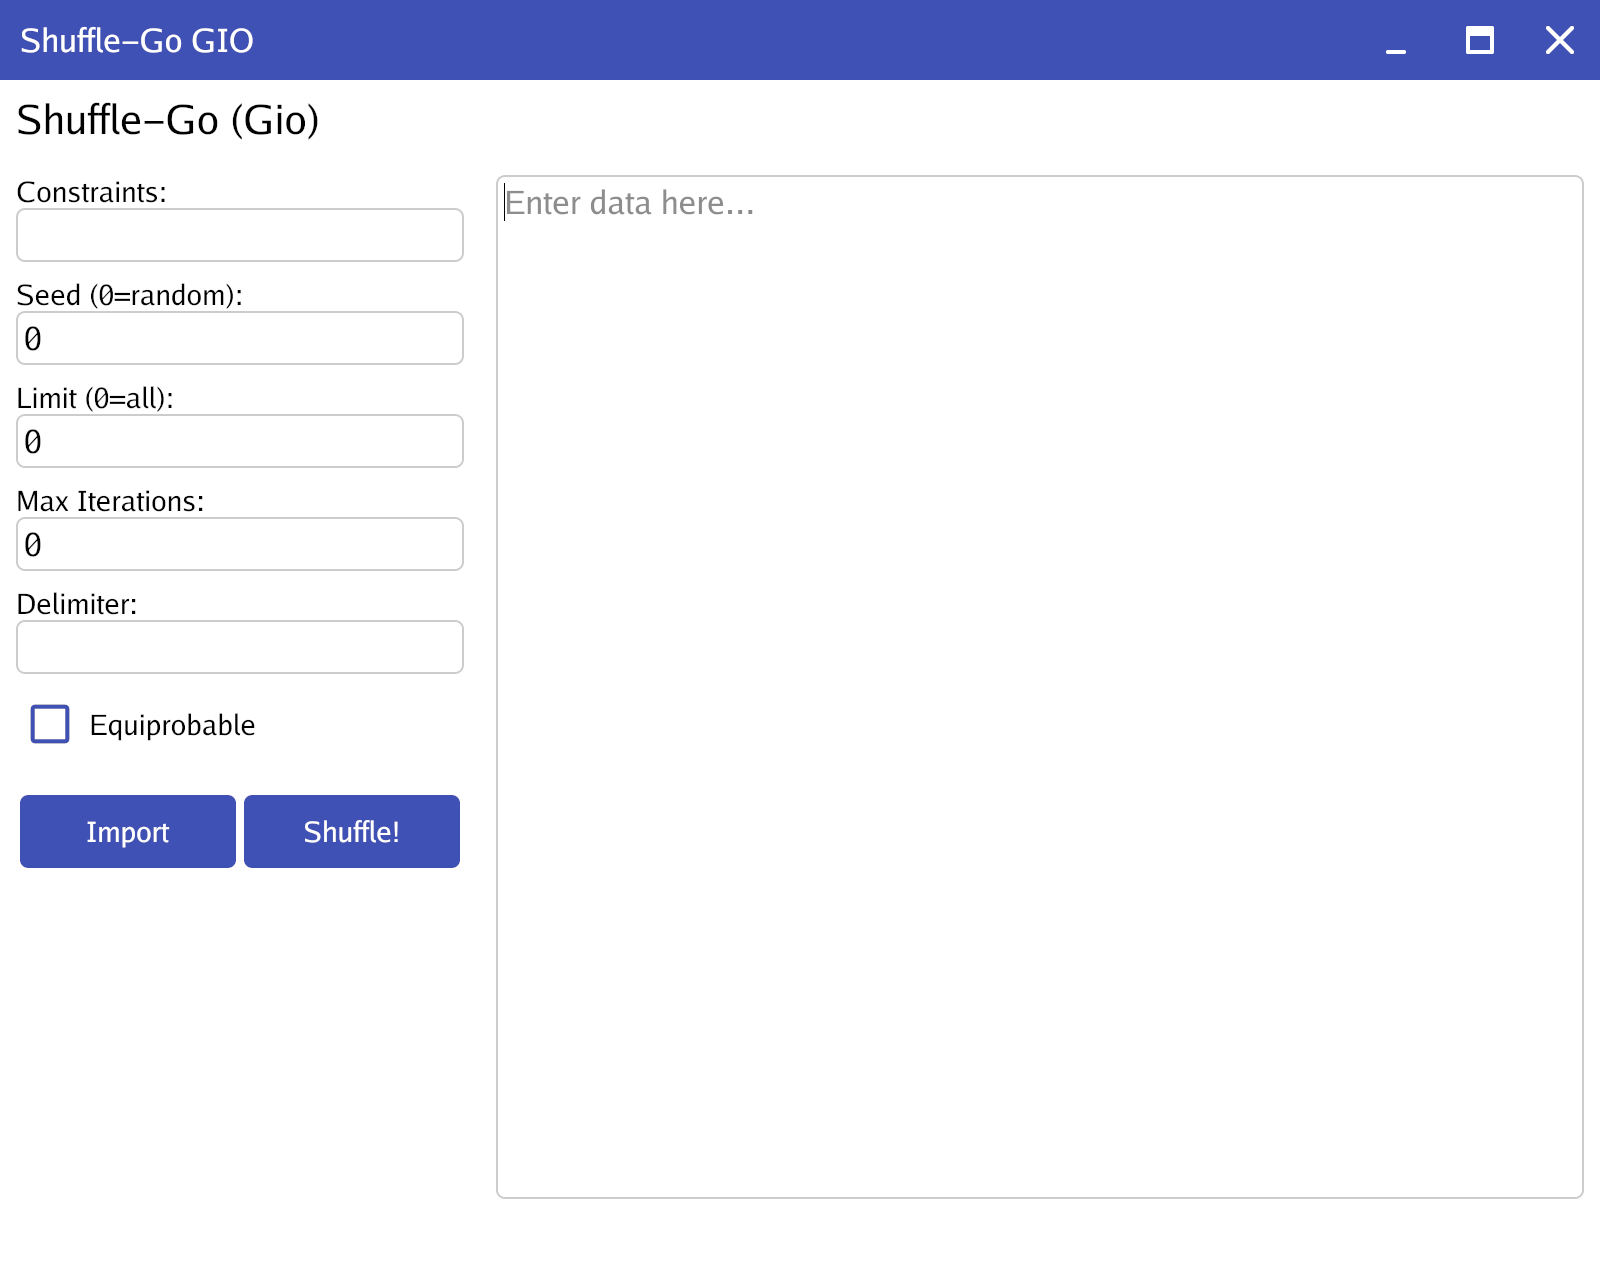
\includegraphics[width=0.6\textwidth]{Gio-ui.png}
  \caption{First Graphical Interface (based on Gio). When Clicking on ``Import'' this app open the native OS file selector. It keeps the look of its ancestor tk version. }\label{gio}
\end{figure}

\begin{figure}
  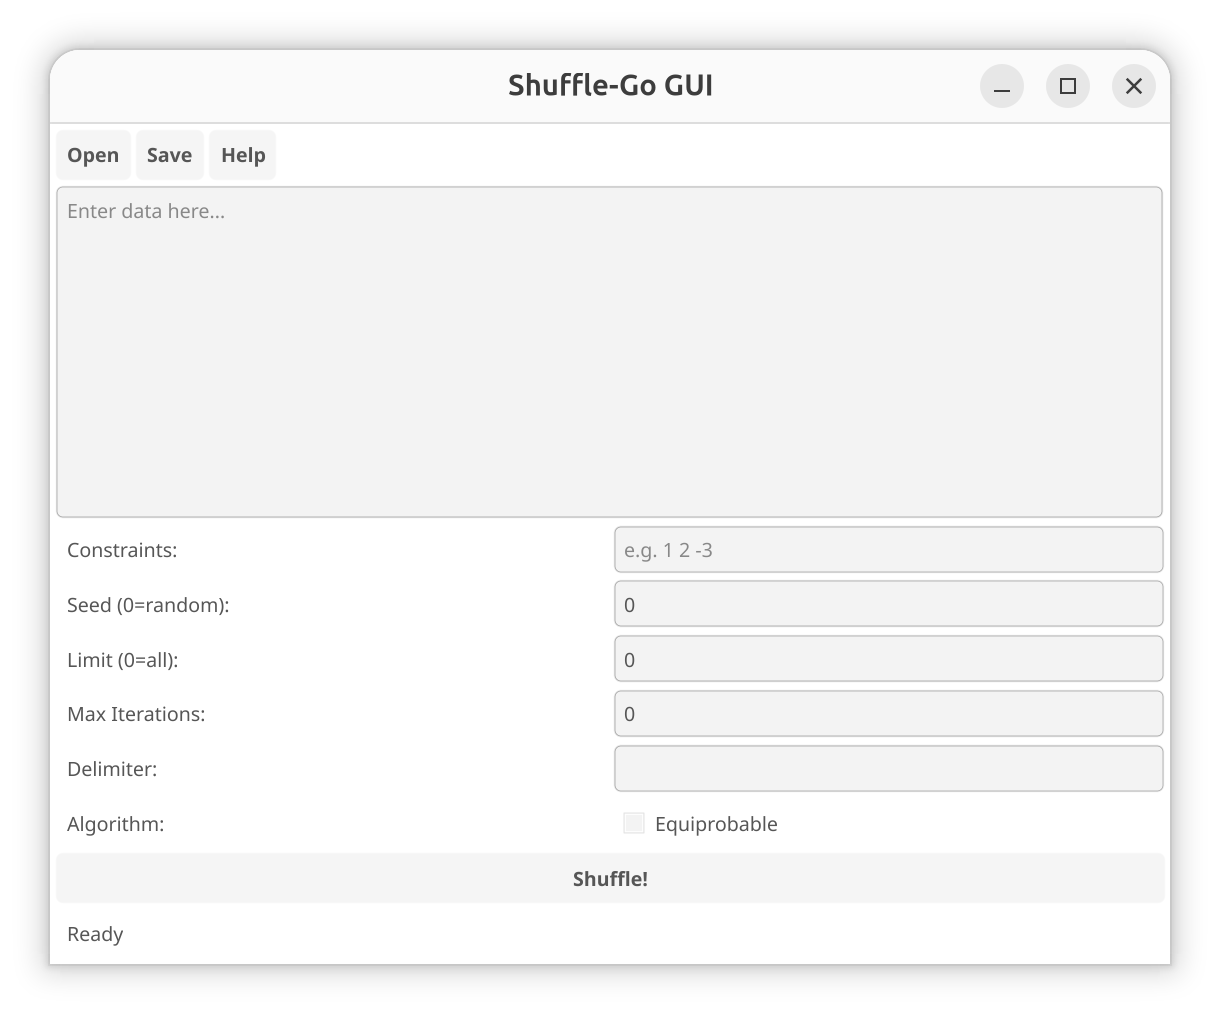
\includegraphics[width=0.6\textwidth]{Fyne-ui.png}
  \caption{Second Graphical Interface (based on Fyne)}\label{fyne}
\end{figure}

\subsection{Go Library}

The core shuffling logic is available as an importable Go package for
integration into larger data-preparation pipelines:

\begin{lstlisting}[caption={Go library usage example}]
import shuffle "github.com/chrplr/shuffle-go"

data, _ := shuffle.LoadData(reader, "")   // auto-detect delimiter
constraints := []shuffle.Constraint{1, -4}
s := shuffle.NewShuffler(data, constraints, 42, 1000, 0)
result, err := s.ShuffleConstructive()
\end{lstlisting}

\subsection{Python Library}

A Python module (\texttt{shuffle.py}) provides the same functionality for
users working in Python:

\begin{lstlisting}[language=Python,caption={Python library usage example}]
from shuffle import load_csv, shuffle_constructive

table = load_csv("stimuli.csv")
result = shuffle_constructive(table, maxrep={0: 1}, mingap={1: 4})
\end{lstlisting}

\noindent
Constraints are passed as dictionaries mapping column index (0-based) to
the constraint value. The module requires Python~3.10 or later and has
no external dependencies.

% -----------------------------------------------------------------------
\section{Availability and Installation}
\label{sec:availability}

\texttt{shuffle-go} is available at
\url{https://github.com/chrplr/shuffle-go} under the GNU General Public
Licence v3 \parencite{fsf1991}. Pre-compiled, self-contained binaries are
provided for Windows (x86-64 and ARM64, as an installer \texttt{.exe} and
a portable \texttt{.zip}), macOS (x86-64 and ARM64, as \texttt{.app}
bundles), and Linux (x86-64 and ARM64, as AppImage and portable
\texttt{.zip}). No runtime environment or additional libraries are
required. On macOS, unsigned binaries may trigger a Gatekeeper security
warning; instructions for bypassing this are provided in the repository.

Users who prefer to build from source require Go~1.24 or later and a C
compiler (the latter is needed only for the GUI components). All three
binaries can be built with:

\begin{lstlisting}[language=bash]
bash build.sh
\end{lstlisting}

\noindent
The Python module (\texttt{shuffle-python/shuffle.py}) requires no
installation beyond copying the file; it has no external dependencies.

% -----------------------------------------------------------------------
\section*{Author Contributions}

C.P. conceptualized the algorithms, implemented them in AWK, Perl and
Python. The translation to Go was performed with the help of Claude
Sonnet 4.6, which was also used to improve a first draft of the current
paper.  Therefore, consistent with current editorial norms
\parencite{natureportfolio2023, springernature2023}, Claude Sonnet 4.6
is listed under Author Contributions rather than as a named author,
because authorship requires the capacity to take accountability for
the work.  Christophe Pallier takes full responsibility for all
content, including the AI-assisted portions.

\section*{Open Practices Statement}

The source code for \texttt{shuffle-go} is openly available at \url{https://github.com/chrplr/shuffle-go}
under the GPLv3 licence. No data were collected for this paper.
%% TODO: add OSF/Zenodo DOI once registered

% -----------------------------------------------------------------------
\printbibliography

\end{document}
